\documentclass[10pt,portrait, twocolumn]{article}
\usepackage{multicol}
\usepackage{calc}
\usepackage[portrait]{geometry}
\usepackage{amsmath,amsthm,amsfonts,amssymb}
\usepackage{times}
\usepackage{color,graphicx,overpic}
\graphicspath{ {images/} }
\usepackage{hyperref}
\usepackage{pgfplots}
\usepackage{esint}
\usepackage{bm}
\usepackage{tikz}
\usepackage{color}
\usepackage{relsize}
\usepackage{datetime}
\usepackage[utf8] {inputenc}
\usepackage[spanish, activeacute] {babel}
\usepackage{IEEEtrantools}
\usetikzlibrary{arrows}
\usepackage{amsmath}

\usepackage{listings}
\usepackage{framed}
\usepackage{color}


\usepackage{pdflscape}

%Evita errores con el paquete de español y escribir flechas entre tikz nodos
\tikzset{
every picture/.append style={
  execute at begin picture={\deactivatequoting},
  execute at end picture={\activatequoting}
  }
}

%\usepackage{draftwatermark}
%\SetWatermarkText{Javier de Martín}
%\SetWatermarkScale{0.8}

% This sets page margins to .5 inch if using letter paper, and to 1cm
% if using A4 paper. (This probably isn't strictly necessary.)
% If using another size paper, use default 1cm margins.
\geometry{top=.5cm,left=.5cm,right=.5cm,bottom=.5cm}
    
\pgfplotsset{
    dirac/.style={
        mark=triangle*,
        mark options={scale=2},
        ycomb,
        scatter,
        visualization depends on={y/abs(y)-1 \as \sign},
        scatter/@pre marker code/.code={\scope[rotate=90*\sign,yshift=-2pt]}
    }
}

\lstset{language=C, % Use Perl in this example
        frame=single, % Single frame around code
        basicstyle=\small\ttfamily, % Use small true type font
%        keywordstyle=[1]\color{Blue}\bf, % Perl functions bold and blue
%        keywordstyle=[2]\color{Purple}, % Perl function arguments purple
%        keywordstyle=[3]\color{Blue}\underbar, % Custom functions underlined and blue
        identifierstyle=, % Nothing special about identifiers                                         
        commentstyle=\usefont{T1}{pcr}{m}{sl}\color{MyDarkGreen}\small, % Comments small dark green courier font
        stringstyle=\color{Purple}, % Strings are purple
        showstringspaces=false, % Don't put marks in string spaces
        tabsize=5, % 5 spaces per tab
        %
        % Put standard Perl functions not included in the default language here
        morekeywords={rand},
        %
        % Put Perl function parameters here
        morekeywords=[2]{on, off, interp},
        %
        % Put user defined functions here
        morekeywords=[3]{test},
       	%
        morecomment=[l][\color{Blue}]{...}, % Line continuation (...) like blue comment
        numbers=left, % Line numbers on left
        firstnumber=1, % Line numbers start with line 1
        numberstyle=\tiny\color{Blue}, % Line numbers are blue and small
        stepnumber=5 % Line numbers go in steps of 5
}

% Turn off header and footer
\pagestyle{empty}

% Redefine section commands to use less space
\makeatletter
\renewcommand{\section}{\@startsection{section}{1}{0mm}%
                                {-1ex plus -.5ex minus -.2ex}%
                                {0.5ex plus .2ex}%x
                                {\normalfont\large\bfseries}}
\renewcommand{\subsection}{\@startsection{subsection}{2}{0mm}%
                                {-1explus -.5ex minus -.2ex}%
                                {0.5ex plus .2ex}%
                                {\normalfont\normalsize\bfseries}}
\renewcommand{\subsubsection}{\@startsection{subsubsection}{3}{0mm}%
                                {-1ex plus -.5ex minus -.2ex}%
                                {1ex plus .2ex}%
                                {\normalfont\small\bfseries}}
\makeatother

\newcommand{\Lagr}{\mathcal{L}}

% Define BibTeX command
\def\BibTeX{{\rm B\kern-.05em{\sc i\kern-.025em b}\kern-.08em
    T\kern-.1667em\lower.7ex\hbox{E}\kern-.125emX}}

% Don't print section numbers
%\setcounter{secnumdepth}{0}


\setlength{\parindent}{0pt}
\setlength{\parskip}{0pt plus 0.5ex}

%My Environments
\newtheorem{example}[section]{Example}
% ---------------------------------------------------------------

\begin{document}

\begin{framed}
	\begin{center}
    	\Large{\underline{ASI}} \\
	\large{Segunda Parte: Seguridad en S.I.} \\
    	\scriptsize{3º Ingeniería de Telecomunicaciones | UPV/EHU}\\
     	%Actualizado por última vez el \today \\
     	"\textsl{Under-promise and over-deliver}." \\
     	%\hspace{5 pt} \\
     	\small{\textbf{Javier de Martín -- 2016/17}}
	\end{center}
\end{framed}

\section{Introducción}

``\textit{The art of war teaches us to rely not on the likelihood of the enemy's not coming, but on our own readiness to receive him; not on the chance of his not attacking, but rather on the fact that we have made our position unassailable.}''\\

\textbf{Amenaza}\footnote{Puede ser causada por usuarios, programas maliciosos, errores de programación, siniestros...}: Condición del entorno del sistema de información que, dada una oportunidad, podría dar lugar a que se produjese un problema de seguridad.\\

Establecer un nivel de seguridad adecuado en un SI es complejo. Hay que definir los servicios a proporcionar, seleccionar las herramientas, monitorización constante...\\

\textbf{Ataque}: Cualquier acción que comprometa la seguridad de cualquier componente de un SI de una organización.\\

\textbf{Servicios de Seguridad}: Un proceso o equipo que lo contiene diseñado para detectar, prevenir o recuperarse de un ataque.\\

\textbf{Mecanismos de Seguridad}: Servicio de procesado o comunicaciones que aumenta la seguridad de los sistemas de procesado o transmisión de información de una organización. Se crean para protegerse de ataques contra la seguridad, y se hace uso de uno o varios mecanismos para proporcionar cada servicio.\\

\textbf{Sevicios de seguridad de OSI} son servicios provistos por una capa de un sistema de comunicaciones, asegurando la seguridad adecuada de los sistemas o transmisiones de datos definidos según la recomendación ITU-T X.800.

\quad Los \textbf{mecanismos de seguridad OSI} son las técnicas o herramientas utilizadas para implementar un servicio de seguridad. Están diseñados para:

	\begin{itemize}
		\item \textbf{Prevenir} ataques que violan la política de seguridad de un sistema
		\item \textbf{Detectar} ataques de violación de la política de seguridad de un sistema.
		\item \textbf{Recuperarse} de un ataque contra la seguridad de un sistema.
	\end{itemize}
	
No existe un único mecanismo capaz de proveer todos los servicios. Los mecanismos pueden ser clasificados como preventivos, detectivos y recuperables.

\section{Fundamentos de Seguridad en los SI}

Un \textbf{Sistema de Información} son los elementos\footnote{Servidores, plataformas de usuario, aplicaciones, red...} que contienen, transportan y sirven información para manipularla.

\subsection{Ataques}
	
Un \textbf{ataque} es una acción contra la seguridad de un sistema que se deriva de una amenaza inteligente. Es un intento deliberado para eludir servicios de seguridad y la política de seguridad de un sistema. Es también cualquier actividad maliciosa que intenta recoger, interrumpir, denegar, degradar o destruir recursos de un Sistema de Información o información. 
	
\quad Un \textbf{ataque pasivo} se basa en la monitorización y atentan contra la confidencialidad. Difíciles de detectar ya que no realizan modificaciones en el sistema.
	
	\begin{itemize}
		\item \textbf{Divulgación de la información}: Se difunde la información obtenida.
		\item \textbf{Análisis de tráfico}: Si la información transcurre encriptada, se puede obtener de ahí información de la frecuencia y distribución del tamaño de la misma.
	\end{itemize}
	
	Un \textbf{ataque activo} implica la modificación o inserción de elementos en el sistema. Tienen características opuestas a los ataques pasivos. Tiene \underline{características opuestas a los ataques pasivos}.
	
		\begin{itemize}
			\item \textbf{Usurpación de identidad}: Se simula ser una entidad distinta con otros privilegios.
			\item \textbf{Retransmisión}: Se vuelven a transmitir secuencias de información, capturadas previamente con objeto de producir un efecto desautorizado.
			\item \textbf{Modificación de mensajes}: Se modifica parte de un mensaje legítimo.
			\item \textbf{Denegación de servicios}: Trata de impedir o degradar el funcionamiento normal del sistema.
		\end{itemize}
	
	\subsection{Servicios}
	
Los \textbf{servicios de seguridad} en OSI son:

	\begin{itemize}
		\item Autenticación
		\item Control de Acceso
		\item Confidencialidad
		\item Integridad de datos
		\item No repudio
	\end{itemize}
	
La \textbf{autenticación entre entidades pares} permite verificar que la entidad es quien dice ser, utilizado en las fases de establecimiento y transferencia de datos. La autenticación del origen de datos no proporciona protección frente a duplicación o modificación. Se emplea en tareas de autorización (concesión de derechos) y contabilidad (control de 

\quad El \textbf{control de acceso} permite proteger los recursos del sistema contra la utilización no autorizada. Para realizar el control de acceso es preciso identificarse. Define perfiles y granularidad.
	
\quad La \textbf{confidencialidad} es la \textbf{protección frente a revelaciones} no autorizadas y ataques pasivos. Cuatro tipos:
	
		\begin{itemize}
			\item \textbf{Orientado a conexión} $\rightarrow$ datos transmitidos durante una conexión. TCP.
			\item \textbf{No orientado a conexión} $\rightarrow$ unidades simples. UDP.
			\item \textbf{De campo selectivo} $\rightarrow$ Campos específicos en una conexión o unidad de datos.
			\item \textbf{Flujo de tráfico} $\rightarrow$ Contra análisis de tráfico.
		\end{itemize}
		
La \textbf{integridad de datos} es la \textbf{protección contra modificaciones} no autorizadas. Se dividen en función del objetivo a proteger (servicio de integridad orientado a conexión o no orientado a conexión) y en función al alcance de la herramienta (servicio con y sin recuperación\footnote{Si se nota que ha habido una modificación se puede pedir una retransmisión del mensaje original.}).
		
\quad \textbf{No repudio} permite proteger contra las posibles negociaciones de acciones realizadas. Hay dos tipos: 
	
		\begin{itemize}
			\item Con prueba de origen $\rightarrow$ Se puede asegurar que el mensaje ha sido enviado por el origen original.
			\item Con prueba de destino $\rightarrow$ Al emisor se le garantiza la recepción en el destino.
		\end{itemize}	
		
La \textbf{disponibilidad} especifica que los sistemas deben estar disponibles siempre\footnote{Como un sistema no puede estar disponible siempre se utilizan sistemas redundantes o detección de fallos.}.
		
\subsection{Mecanismos}

Los \textbf{mecanismos de seguridad de OSI} son:

	\begin{itemize}
		\item \textbf{Específicos}: Técnicas destinadas a facilitar un servicio\footnote{Por ejemplo: Cifrado, firma digital, control de acceso, integridad, intercambio de autenticación, relleno de tráfico, control de encaminamiento y certificación}.
		\item \footnote{Generalizados}: Pueden considerarse como aspectos de gestión de seguridad (relacionados directamente con el nivel de seguridad requerido)\footnote{Por ejemplo: confianza, etiquetas de seguridad, detección, recuperación...}
	\end{itemize}
	
También es interesante considerar mecanismos a distintos niveles:

	\begin{itemize}
		\item \textbf{Mecanismos a nivel de Red}: Se autentica y cifra todo el tráfico de red, se protege a todas las aplicaciones, requieren la misma solución en todos los nodos, IPv6 e IPsec fueron diseñados con ello en mente. Hay soluciones parciales, entre routers de la organización VPN.
		\item \textbf{Mecanismos a nivel de Aplicación}\footnote{PCP, SSH, HTTPS, SSL...}: Dado que no hay mecanismos globales, se buscan soluciones para cada una de las aplicaciones que nos interesa.
	\end{itemize}
	
	\begin{figure}[ht!]
	\centering
	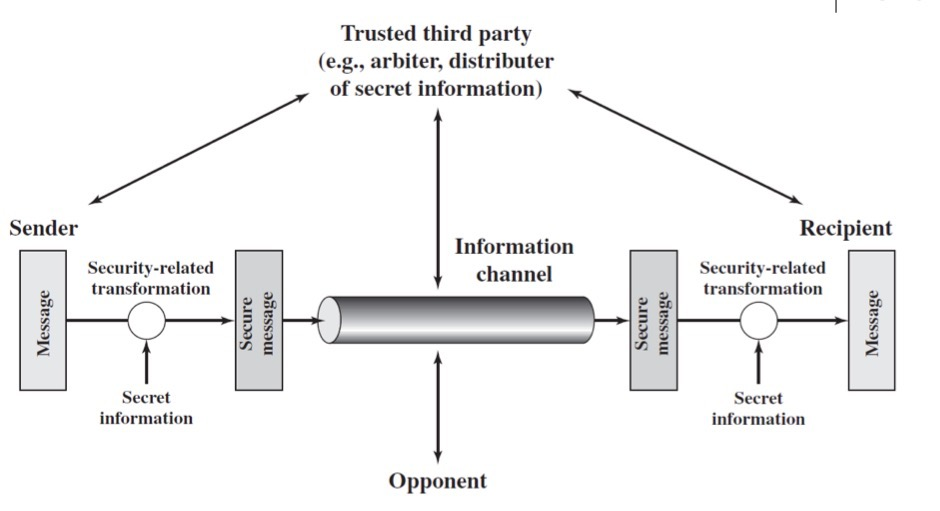
\includegraphics[width = .5\textwidth]{images/ModeloSeguridad}
	\caption{Modelo de Seguridad de Red}
	\label{table:Planta1}
	\end{figure}
	
\textcolor{red}{Explicar dibujo}

	\begin{figure}[ht!]
	\centering
	\includegraphics[width = .5\textwidth]{images2/Modelo}
	\caption{Modelo de Seguridad para Acceso a Red}
	\label{table:Planta1}
	\end{figure}
	
\textcolor{red}{Explicar dibujo}

	\begin{figure}[ht!]
	\centering
	\includegraphics[width = .15\textwidth]{images2/Triada}
	\caption{Triada de Seguridad}
	\label{fig:Triada}
	\end{figure}
	
La NIST define la seguridad como la triada (figura \ref{fig:Triada}) CIA: Confidentiality, Integrity y Availability:

	\begin{itemize}
		\item \textbf{Confidencialidad}: Protección del acceso (o revelación) a la información solo para personas autorizadas, incluyendo medios para proteger privacidad e información de propietario. Una pérdida de confidencialidad supone la revelación no autorizada de información.
		\item \textbf{Integridad}: Protección frente a modificación o destrucción de información de forma no autorizada (incluye no repudio y autenticidad). Una pérdida de integridad supone la modificación o destrucción no autorizada de información.
		\item \textbf{Disponibilidad}: Asegurar el acceso y la utilización a tiempo y de forma confiable a la información. Una pérdida de disponibilidad supone la interrupción en el acceso o utilización de una información o sistema de información.
		\item \textbf{Autenticidad}: Propiedad de ser genuino y con capacidad para ser verificado y confiable. Confiabilidad en la validez de una transmisión, de un mensaje o del originador de un mensaje. Que se pueda verificar que los usuarios son quienes dicen ser, o que las entradas a un sistema proceden de una fuente confiable.
		\item \textbf{Contabilidad}: Como no es posible que los sistemas sean completamente seguros, las partes autorizadas deberían disponer de mecanismos para trazar eventos de seguridad. Los sistemas deben almacenar registros de sus actividades para permitir análisis forenses posteriores para ayudar en la resolución de conflictos. Proporciona no repudio, disuasión, detección y prevención de intrusión, y posibilita recuperación y acciones legales posteriores.
	\end{itemize}
	
\begin{figure}[ht!]
	\centering
	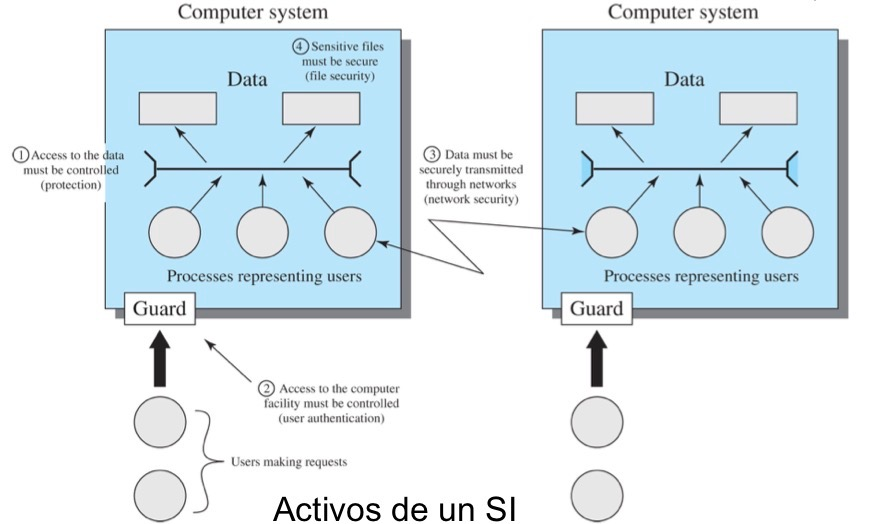
\includegraphics[width = .15\textwidth]{images/Activos}
	\caption{Activos, amenazas y ataques}
	\label{fig:Triada}
	\end{figure}
\textcolor{red}{Explicar dibujo}


	\begin{itemize}
		\item \textbf{Amenazas}: "\textit{Condición del entorno de sistema de información que, dada una oportunidad, podría dar lugar a que se produjese una violación de la seguridad}".
		\item \textbf{Ataque}: "\textit{Un ataque es la realización de una amenaza}".
	\end{itemize}
	
Una \textbf{amenaza a la seguridad} es la posibilidad de violación de seguridad, que existe cuando una entidad, circunstancia que puede causar daños. Un peligro que se deriva de una posible explotación de una vulnerabilidad. Para estudiar los tipos de amenazas se suele partir de la consideración que la función de un SI es proporcionar información, se considera que hay un flujo de información de una fuente a un destino.

	\begin{figure}[ht!]
	\centering
	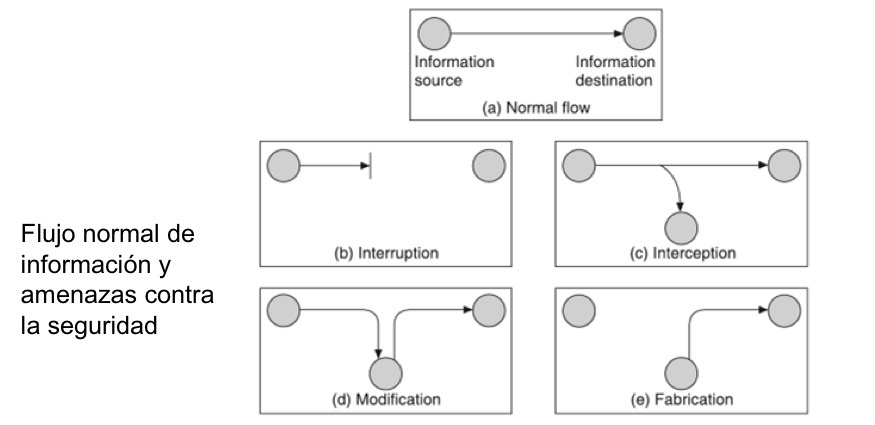
\includegraphics[width = .15\textwidth]{images/Amenaza}
	\caption{Amenazas a la seguridad}
	\label{fig:Triada}
	\end{figure}

\textcolor{red}{Explicar dibujo}




\section{Técnicas Criptográficas}

	\subsection{Introducción a la criptografía}
	
	\begin{itemize}
		\item \textbf{Esteganografía} tiene como objetivo ocultar la existencia de un mensaje.
		\item \textbf{Criptografía}: Objetivo es ocultar el significado del mensaje, el proceso se conoce como codificación.
		\item \textbf{Criptología}: Ciencia que trata los problemas teóricos relacionados con la seguridad en el intercambio de mensajes en clave entre un emisor y un receptor a través de un canal de comunicaciones. Criptografía + Criptoanálisis.
		\item \textbf{Criptografía}: Técnicas de cifrado o codificado destinadas a alterar las representaciones lingüísticas de mensajes con el fin de hacerlos ininteligibles a receptores no autorizados. Tradicionalmente asociada sólo al cifrado. Actualmente es parte de la criptología que se encarga del estudio de los algoritmos, protocolo criptográficos y sistemas que se utilizan para proteger la información y dotar de seguridad a las comunicaciones y las entidades que se comunican.
	\end{itemize}
	
	\begin{figure}[ht!]
	\centering
	\includegraphics[width = .45\textwidth]{images2/Fundamentos}
	\caption{Fundamentos de la criptografía}
	\label{fig:Triada}
	\end{figure}

\textbf{Elementos clave del sistema}: 
	\textcolor{red}{Terminar}
	
	\begin{itemize}
		\item \textbf{Texto en claro}:
		\item \textbf{Texto cifrado}:
		\item \textbf{Clave de cifrado}: $K_{A}$
		\item \textbf{Clave de descifrado}: $K_{B}$
	\end{itemize}
	
Los \textbf{sistemas criptográficos} se caracterizan en función de:
	
	\begin{itemize}
		\item Tipo de operaciones utilizadas para transformar el plaintext en ciphertext: sustitución y transposición.
		\item Número de claves utilizadas: simétrica y asimétrica.
		\item Forma en la que se procesa el plaintext: Bloque y stream.
	\end{itemize}
	
	Tipos básicos de cifrado en función del tipo de operaciones:
	
	\begin{itemize}
		\item Sustitución: Las unidades de texto plano son sustituidas con texto cifrado siguiendo un sistema regular. Las unidades pueden ser una sola letra o grupos más grandes. El receptor descifra el texto realizando la operación inversa. Hay varios tipos:
			\begin{itemize}
				\item Simple: Opera sobre letras simples. Hay mono alfabético, si la sustitución es simple para todo el mensaje, y polialfabético, si utiliza diferentes sustituciones en diferentes partes de un mensaje.
				\item Poligráfico: Opera sobre grupos de letras.
			\end{itemize}
		\item Transposición: Las unidades del texto plano son cambiadas usando una ordenación diferente y normalmente bastante compleja, pero las unidades en sí mismas no son modificadas. 
	\end{itemize}
	
Criptografía de \textbf{clave secreta o simétrica}: Se utiliza la misma clave para cifrar y descifrar.

	\begin{equation*}
		K_A = K_B = K_{AB} \hspace{10pt} K_{AB} (K_{AB}(m)))
	\end{equation*}
	
	La clave es \textbf{secreta} ($K_{AB}$) es conocida por los dos participantes de la comunicación.\\
	
	\begin{figure}[ht!]
	\centering
	\includegraphics[width = .45\textwidth]{images2/Asimetrica}
	\caption{Criptografía de clave secreta o simétrica}
	\label{fig:Triada}
	\end{figure}	
	
	\textcolor{red}{Terminar}
	
Criptografía de \textbf{clave pública o asimétrica}: Cada usuario cuenta con un par\footnote{Por ejemplo, para un usuario Alice su par sería $K_{A}^{+}$/$K_{A}^{-}$.} de clave pública ($K^{+}$)/privada ($K^{-}$). Dada la clave pública ($K^{+}$), es computacionalmente inviable obtener la clave privada ($K^{-}$). La clave privada es secreta y por tanto, conocida únicamente por el propietario legítimo de la misma, mientras que la clave pública es pública, y por tanto conocida por todos.\\

	\begin{figure}[ht!]
	\centering
	\includegraphics[width = .45\textwidth]{images2/Simetrica}
	\caption{Criptografía de clave pública o asimétrica}
	\label{fig:Triada}
	\end{figure}
	\textcolor{red}{Terminar}

Todo lo que se cifra con la clave pública únicamente puede ser descifrado con la correspondiente clave privada y vice-versa.

	\begin{equation*}
		K^+(K^-(m))) = m \hspace{10pt} \text{ó} \hspace{10pt} K^-(K^+(m))) = m
	\end{equation*}
	
Para garantizar la confidencialidad de los mensajes enviados, todos los emisores han de cifrar los mensajes con clave pública del usuario de destino ($K_{X}^{+}$), conocida por todos,  y sólo será el usuario de destino que podrá descifrar el mensaje con su clave privada ($K_{X}^{-}$). El proceso sería el siguiente:

\begin{eqnarray*}
&\text{Alice:}& m \rightarrow K_{B}^{+}(m)\\
&\text{Bob:}& K_{B}^{-} \{ K_{B}^{+} (m) \} = m
\end{eqnarray*}

	
\textbf{Criptoanálisis} es la parte de la criptología que se dedica al estudio de sistemas criptográficos con el fin de encontrar debilidades en los sistemas y romper su seguridad. Buscar romper o forzar el código. Hay varios tipos de ataques según el conocimiento previo del atacante:

	\begin{itemize}
		\item \textbf{Ataques \textit{ciphertext-only}}: Cuando sólo se dispone del texto cifrado. Por ejemplo: Fuerza bruta, análisis de frecuencias o método Kasiski.
		\item \textbf{Ataque \textit{known-plaintext}}: El atacante conoce el texto original. En ocasiones, el atacante conoce una parte del texto o alguna palabra probable.
		\item \textbf{Ataque \textit{chosen-plaintext}}: El atacante tiene la capacidad de definir un texto y obtener el correspondiente texto cifrado. El objetivo es poder descifrar textos que se descicfren e ese descifrador. Si un sistema es seguro frente a ataques \textit{chosen-plaintext} también es seguro frente a ataques \textit{known-plaintext} y \textit{ciphertext-only}.
	\end{itemize}

	
	\subsection{Cifrado}
	
El \textbf{cifrado} es la puesta en clave (\textit{ciphertext}) de un texto (\textit{plaintext}) mediante una función parametrizada por una clave. Previene ataques contra la confidencialidad.

	\begin{figure}[ht!]
	\centering
	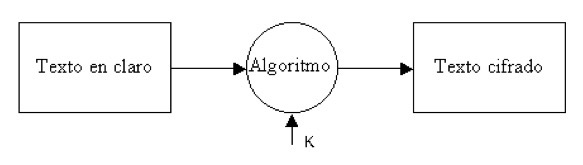
\includegraphics[width = .45\textwidth]{images/Cifrado}
	\caption{Cifrado}
	\label{fig:Triada}
	\end{figure}
	
El criptoanálisis es la ciencia que estudia los sistemas que permiten desbaratar textos cifrados y obtener los correspondientes textos en claro.\\

Los algoritmos de cifrado más antiguos hacen uso de criptografía simétrica.\\

\textcolor{red}{Tamaño de claves para proporcionar un nivel de seguridad similar en algoritmos de cifrado. \textbf{Tabla de bits cifrado no entiendo}}
	
\subsection{Códigos de Autenticación de Mensaje (MAC)}

Permiten proteger la integridad y autenticidad de origen de los mensajes. Comprueban que el origen del mensaje es quién dice ser y que dicho mensaje no ha sido modificado durante su transmisión. Pueden considerarse sinónimos, si un mensaje es modificado durante su transmisión, ya no procede de su emisor légitimo sino de quien lo modificó.\\
\quad A veces puede ser necesario garantizar la integridad del mensaje pero no su confidencialidad.\\

	\begin{figure}[ht!]
	\centering
	\includegraphics[width = .45\textwidth]{images2/Autenticacion}
	\caption{Autenticación de Origen}
	\label{fig:Triada}
	\end{figure}
		\textcolor{red}{Explicar}

Una \textbf{función \textit{hash}}\footnote{Por ejemplo los códigos CRC} $h$ es una función que mapea cadenas de bits de longitud arbitraria a cadenas de longitud fija de $n$ bits (huella dactilar), es una función resumen y es de un único sentido. Dada una función hash $h$ y una entrada $x$, la salida $h(x)$ es computacionalmente sencilla de calcular. Se puede ir del texto al resumen pero en sentido inverso es imposible, una función hash no es reversible. Dado un valor $y$, es computacionalmente inviable encontrar un valor de $x'$ de forma que $h(x')=y$ por tanto no habrá colisiones.\\

\textbf{MAC} (\textit{Message Authentication Code}) es un código que permite la autenticación de mensajes mediante técnicas criptográficas de clave simétrica. Los algoritmos de MAC toman como entrada dos parámetros (mensaje y clave simétrica) y generan una salida de longitud fija con la característica de que es computacionalmente inviable producir la misma salida sin conocer la clave. 
	\begin{center}
		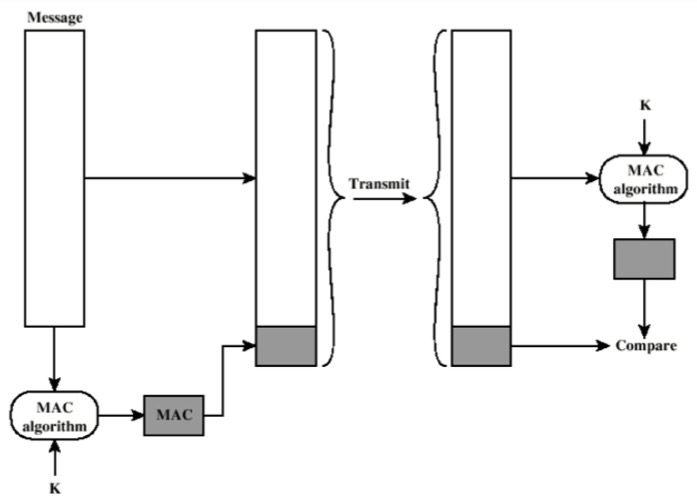
\includegraphics[width = 0.35\textwidth]{images/MAC}
	\end{center}
	\textcolor{red}{Terminar}
	
Un \textbf{ejemplo de código MAC} es HMAC (\textit{Hash-based Message Authentication Code}) y es un tipo específico de códigos MAC, el algoritmo utilizado para calcular el código MAC se basa en la utilización de funciones hash en lugar de, por ejemplo, algoritmos de cifrado.
	
		\begin{center}
		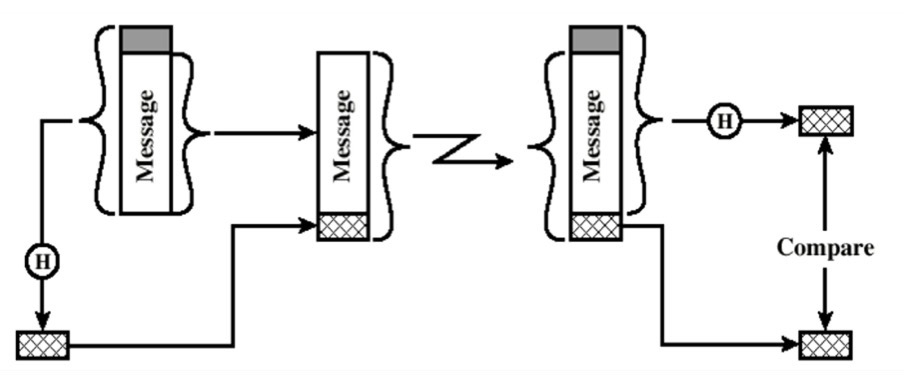
\includegraphics[width = 0.25\textwidth]{images/HMAC}
	\end{center}
	
\textbf{Características de los códigos de autenticación de mensajes}:

	\begin{itemize}
		\item Compresión: Mapean una entrada de longitud fija finita arbitraria a una salida de longitud finita fija.
		\item Facilidad de cómputo: Dada una función hash $h$ y una entrada $x$, la salida $h(x)$ es computacionalmente sencilla de calcular.
		\item Unidirecional (no reversible): Dado un valor $y$, es computacionalmente inviable encontrar un valor $x'$ de forma que $h(x')=y$.
		\item Sin colisiones: Es computacionalmente inviable encontrar dos entradas $x$ y $x'$ distintas de forma que $h(x) = h(x')$.
	\end{itemize}
	
	\subsection{Firmas Digitales}
	
Técnica criptográfica análoga a las firmas hechas a mano. Garantiza la integridad o autenticación de origen de un mensaje. Es verificable, no falsificable. El destinatario puede demostrarle a alguien que el origen, y no otra persona (incluyendo el destinatario), ha firmado el documento. Resumen (\textit{hash}) del mensaje cifrado.

	\begin{figure}[ht!]
	\centering
	\includegraphics[width = .5\textwidth]{images2/GeneracionFirma}
	\caption{Generación de firma digital}
	\label{table:Planta1}
	\end{figure}
	
La verificación separa el mensaje de la firma. Con el algoritmo de descifrado y la clave pública de A se extrae el resumen. ¿Por qué tiene que haber un resumen criptográfico? Para evitar conseguir dos resúmenes que sean iguales.
	
	\begin{figure}[ht!]
	\centering
	\includegraphics[width = .5\textwidth]{images2/VerificacionFirma}
	\caption{Verificación de firma digital}
	\label{table:Planta1}
	\end{figure}
	
No se puede autenticar el origen con el hash.

\begin{tabular}{llll}
Crypto Primitive Security Goal & Hash & MAC               & Digital Signature  \\
Integrity                             & Yes  & Yes               & Yes                \\
Authentication                        & No   & Yes               & Yes                \\
Non-Repudiation                       & No   & No                & Yes                \\
Kind of Keys                          & None & Claves simétricas & Claves asimétricas
\end{tabular}	
	
	\subsection{Frescura de Mensajes}
	
Incluso cifrando un mensaje y autenticándolo (mediante código MAC o firma digital) todavía es posible que un atacante intercepte un mensaje legítimo y lo repita más tarde haciéndose pasar por el emisor legítimo (ataque de repetición de mensajes). Es necesario garantizar la frescura de los mensajes.

\quad Un \textbf{ataque de repetición de mensajes} consiste en que el destinatario cree que ha recibido un nuevo mensaje del origen cuando en realidad se trata de un mensaje antiguo repetido por un intermediario.

	\begin{figure}[ht!]
	\centering
	\includegraphics[width = .5\textwidth]{images2/Repeticion}
	\caption{Ataque de Repetición de Mensajes}
	\label{table:Planta1}
	\end{figure}
	
\textbf{Mecanismos de Frescura}:

	\begin{itemize}
		\item \textbf{Sellos de tiempo}: Genera datos que identifican el momento en el que se crearon los datos. Pueden estar basados en la utilización de relojes o en sellos de tiempo lógicos (números de secuencia). ?`Cómo funciona? El generador del mensaje incluye la hora/fecha de generación del mensaje (sello de tiempo) en el mensaje original. Cuando el destinatario recibe el mensaje, compara el sello de tiempo incluido en el mismo con la hora/fecha actual. Si el retardo del mensaje es mayor que el retardo normal en la red de comunicaciones se descarga el mensaje (se trata de un mensaje repetido). Tiene una desventaja, tanto el origen como el destino tienen que mantener sus relojes sincronizados.
		\item \textbf{Nonces/Testigos}: Número que se introduce para una utilización única (one-time identification). Normalmente, es un número generado aleatoriamente. Refleja la frescura si asumimos que se generan números que no han sido usado antes. Son valores únicos e impredecibles. A $N1$ se le denomina reto (\textit{challenge})
		
			\begin{figure}[ht!]
			\centering
			\includegraphics[width = .4\textwidth]{images2/Nonces}
			\caption{Nonces}
			\label{figure:Planta1}
			\end{figure}
			
		\item \textbf{Unilateral Symmetric Key}:
		
			\begin{itemize}
				\item Autenticación con sello de tiempo generado por A:  Origen y destino tienen los relojes sincronizados, el destino sólo acepta mensajes durante un cierto período de tiempo.
					\begin{figure}[ht!]
					\centering
					\includegraphics[width = .2\textwidth]{images2/USK}
					\caption{Autenticación con sello de tiempo generado por el origen}
					\label{figure:Planta1}
					\end{figure}
					
				\item Autenticación unilateral con \textit{nonce}:
					
					\begin{figure}[ht!]
					\centering
					\includegraphics[width = .2\textwidth]{images2/USK2}
					\caption{Autenticación unilateral con nonce}
					\label{figure:Planta1}
					\end{figure}
			\end{itemize}
			
			\item \textbf{Mutual Symmetric Key}: Con nonces
			
				\begin{figure}[ht!]
				\centering
				\includegraphics[width = .2\textwidth]{images2/MSK}
				\caption{Mutual Symmetric Key con nonces}
				\label{figure:Planta1}
				\end{figure}
	\end{itemize}
	
	\subsection{Distribución de Claves}

Está obligatoriamente ligado al proceso de autenticación. No tiene sentido establecer una clave con un usuario no autenticado, \textit{?`Es realmente el usuario con el que me quiero comunicar?}. No tiene sentido autenticar a un usuario y no establecer una clave, \textit{?`Una vez finalizado el proceso de autenticación cómo sé que el usuario con el que me estoy comunicando es el mismo previamente autenticado?}.

\quad La \textbf{criptografía de clave simétrica}: Tiene varios problemas, \textit{?`Cómo pueden dos entidades establecer una clave secreta compartida a través de la red no segura?} Se requiere una clave por cada par de usuarios. Para $n$ participantes hay $n \frac{n-1}{2}$ claves. La solución es el centro de distribución de claves (\textit{KDC}) actuando como intermediario en el que confían las dos entidades que quieren establecer una clave compartida entre ambas.\\

	\begin{figure}[ht!]
		\centering
		\includegraphics[width = .2\textwidth]{images2/Claves}
		\caption{Comparativa del número de claves}
		\label{figure:Planta1}
		\end{figure}

\textcolor{red}{Explicar dibujo}

En el \textbf{centro de distribución de claves} (KDC) cada usuario registrado en el sistema comparte una calve secreta con el KDC:

	\begin{itemize}
		\item $K_{A, KDC}$: Clave compartida entre Alice y el KDC.
		\item $K_{B, KDC}$: Clave compartida entre Bob y el KDC.
	\end{itemize}
	
	\begin{figure}[ht!]
	\centering
	\includegraphics[width = .4\textwidth]{images2/KDC}
	\caption{Key Distribution Center}
	\label{figure:Planta1}
	\end{figure}
	
KDC, establecimiento de clave $K'$ como clave de sesión para comunicación segura entre origen y destino.
	
	\begin{figure}[ht!]
	\centering
	\includegraphics[width = .35\textwidth]{images2/KDC2}
	\caption{Establecimiento de una clave}
	\label{figure:Planta1}
	\end{figure}
	
Kerberos es uno de los sistemas de distribución de claves más populares. El KDC consta de 2 servidores, \textit{Authentication Server} (AS) y \textit{Ticket Granting Server} (TGS). En cuanto a \textbf{escalabilidad} permite la existencia de diferentes dominios (\textit{realms}). Los KDCs de los diferentes dominios establecen asociaciones de seguridad entre sí. La \textbf{autenticación} de usuario se realiza en 2 fases:

	\begin{itemize}
		\item Fase de autenticación: El usuario se autentica frente al AS de Kerberos. Obtiene un \textit{Ticket Granting Ticket} (TGT), el cual es una especie de ticket maestro que identifica al usuario como ya autenticado. 
		\item Fase de emisión de tickets: El usuario obtiene del TGS de kerberos un ticket de servicio, el cual es la credencial que ha de presentar al usuario remoto frente al que se quiere autenticar.
	\end{itemize}
	
Este mecanismo de autenticación permite implementar mecanismos de \textit{Single-Sign On}, gracias al TGT el usuario puede obtener todos los tickets de servicio que desee sin volver a autenticarse frente al AS.

	\begin{figure}[ht!]
	\centering
	\includegraphics[width = .4\textwidth]{images2/Kerberos}
	\caption{Operación de Kerberos}
	\label{figure:Planta1}
	\end{figure}
	
\textcolor{red}{COmentar con texto la figura}
	
		\begin{figure}[ht!]
	\centering
	\includegraphics[width = .4\textwidth]{images2/Kerberos2}
	\caption{Operación de Kerberos}
	\label{figure:Planta1}
	\end{figure}
	
\textcolor{red}{Comentar la imagen}\\

En KDC se demuestra la identidad una vez. En TGS se solicitan los servicios con el ticket.

\textcolor{red}{Si tienes un certificado por ti mismo significa que eres una autoridad certificadora.}\\

Primera flecha, Viaja en claro $A$ le dice al $KDC$ que quiere hablar con el $TGS$. Le devuelve un ticket y la clave $A-TGS$.

\quad $A$ le envía al TGS su ticket y servicio que solicita.\\

\textcolor{red}{Un \textbf{certificado} es una identidad con una clave pública firmados por una autoridad.}\\

La criptografía de clave pública tiene un problema, \textit{Cuando Bob obtiene la clave pública de Alice, ?`Cómo puede estar seguro de que es realmente la clave pública de Alice y no de otro usuario intentando hacerse pasar por Alice?} Se puede dat un ataque \textit{Man in the Middle}.

\begin{figure}[ht!]
	\centering
	\includegraphics[width = .4\textwidth]{images2/MITM}
	\caption{Man in the Middle}
	\label{figure:Planta1}
	\end{figure}

La \textbf{solución} a los positbles ataques MiTM es la CA (\textit{Certification Authority}). Está basado en el uso de Autoridades de Certificación y servicios de directorio. Un certificado digital es un documento digital firmado por una Autoridad de Certificación de confianza que asocia una clave pública a una identidad. Si dos usuarios disponen de certificados emitidos por diferentes CAs es preciso construir una vía de certificación. Claves públicas de CAs dentro de los navegadores.

\quad Un \textbf{certificado digital} (X.509) es un documento firmado por una Autoridad de Ceritficación de confianza que asocia una clave pública a una identidad.

\quad Si dos usuarios disponen de certificados emitidos por diferentes CAs es preciso construir una \textbf{vía de certificación}.

\quad \textcolor{red}{Un usuario $A$ $E^{-}_{AC_{1}} \{ A, E^{+}_{A} \}$ con una AC1 y uno B $E^{-}_{AC_{2}} \{ B, E^{+}_{B} \}$ con una AC2 certificados por dos autoricades diferentes ya que uno no le vale al del otro, entonces una autoridad certificadora tiene que verificar la identidad de la otra autoridad verificadora. Por ejemplo para el usuario A, tiene que verificar la identidad de la AC2 como $E^{-}_{AC_{1}} \{ AC2, E^{+}_{AC2} \}$}.

\quad Una CA necesita una \textbf{prueba de identidad}\footnote{Clave pública y la clave pública firmada con la clave privada $\rightarrow$ $E^{-}_{AC} \{  A, E_{A}^{+} \}$} de un $E(\text{persona}, \text{router})$ para poder crear un certificado\footnote{Este certificado contiene la clave pública de E firmada digitalmente por CA} que vincule a E a su clave pública.\\

El certificado será la pareja identidad clave pública firmada por la autoridad certificadora:

\begin{equation*}
E^{-}_{AC} = \{A, E^{+} _{A}\}
\end{equation*}

	\begin{figure}[ht!]
	\centering
	\includegraphics[width = .4\textwidth]{images2/CA}
	\caption{Emisión de certificados por la CA}
	\label{figure:Planta1}
	\end{figure}



	
	
%\textcolor{red}{}	


Cuando un usuario $B$ quiere comunicarse con un usuario $A$ le solicita la clave pública. Obtiene el certificado de $A$, aplica la clave pública CA al certificado de $A$.

	\begin{figure}[ht!]
	\centering
	\includegraphics[width = .4\textwidth]{images2/BA}
	\caption{Petición de B a A por su certificado}
	\label{figure:Planta1}
	\end{figure}
	
\textbf{Certificados cruzados}. Dos usuarios $A$ y $B$ con certificados emitidos por \texttt{CA1} y \texttt{CA2} no pueden verificar los certificados de manera segura por que no tienen los certificados de la otra CA.

	\begin{itemize}
		\item \texttt{A} dispone de:
			\begin{itemize}
				\item Certificado de \texttt{CA1}: $E_{CA1}^- \{ CA1, E^+_{CA1} \}$
				\item Certificado de \texttt{B} emitido por \texttt{CA2}: $E_{CA2}^- \{ B, E^+_{B} \}$
			\end{itemize}
		\item \texttt{B} dispone de:
			\begin{itemize}
				\item Certificado de \texttt{CA2}: $E_{CA2}^- \{ CA2, E^+_{CA2} \}$
				\item Certificado de \texttt{A} emitido por \texttt{CA1}: $E_{CA1}^- \{ A, E^+_{A} \}$
			\end{itemize}
	\end{itemize}	
	
El protocolo Diffie-Hellman es un \textbf{protocolo de establecimiento de claves} entre partes que no han tenido contacto previo utilizando un canal inseguro y de manera anónima (no autenticada). Se emplea como medio para acordar claves simétricas que se emplearán para el cifrado de una sesión. A pesar de no ser autenticado provee las bases para protocolos autenticados. Está sujeto a ataque de hombre de en medio por tanto habrá que usar una autenticación por encima.

	\begin{figure}[ht!]
	\centering
	\includegraphics[width = .4\textwidth]{images2/Diffie}
	\caption{Protocolo Diffie-Hellman}
	\label{figure:Planta1}
	\end{figure}
	
\textcolor{red}{Explicación: Existe una parte común \texttt{g}}	

	\begin{figure}[ht!]
	\centering
	\includegraphics[width = .4\textwidth]{images2/DH}
	\caption{Funcionamiento del Protocolo Diffie-Hellman}
	\label{figure:Planta1}
	\end{figure}

\subsection{Criptografía Simétrica y Asimétrica}

La \textbf{criptografía simétrica} tiene un espacio de claves $\geq 128$ bits, la vida de las claves es muy corta, la velocidad de firma es muy alta, la seguridad reside en la de la propia clave y el tamaño del mensaje no importa\footnote{Con algoritmos de bloque se puede firmar todo lo que sea}. 

\quad Para la \textbf{criptografía asimétrica} el espacio de claves es $\geq 1024$ bits\footnote{Tamaño en bits que tiene el entero resultado de multiplicar dos números primos grandes}, la vida de éstas es larga, la velocidad de la firma es lenta, la seguridad reside en la dificultad computacional de encontrar la clave privada a partir de la clave pública y el tamaño del mensaje es menor que la longitud de la clave\footnote{Si por ejemplo el espacio de claves es de 1024 bits se pueden firmar mensajes de como máximo 128 bits}.\\

En la práctica se usa \textbf{criptografía híbrida} que utiliza dos algoritmos:

	\begin{itemize}
	\item Algoritmo de calve pública: Es más seguro y se usa para el cifrado en el envío de la clave simétrica.
	\item Algoritmo de clave simétrica: Se utiliza en el cifrado del mensaje y reduce el coste computacional.
	\end{itemize}

	\begin{figure}[ht!]
	\centering
	\includegraphics[width = .4\textwidth]{images2/Hibrida}
	\caption{Funcionamiento de la criptografía híbrida}
	\label{figure:Planta1}
	\end{figure}

	
Se genera una clave $S$ que se usa para cifrar el mensaje $M$. La clave $S$ se firma con la pública de $B$ certific. Tiene un problema ya que no se firma y se desconoce quién lo envía, si se quisiera firmar habrá que añadir el hash del mensaje crifrado con la clave privada del origen.\\

\textcolor{red}{Si dicen que A y B tienen certificado están diciendo que la correspondencia entre clave pública y propietario están verificadas, por tanto no puede haber ataque de MITM.}\\

\subsection{Seguridad en SI}

\subsubsection{Seguridad en Dispositivos Finales}

La seguridad en equipos finales se consigue utilizando un SO seguro, eligiendo buenas contraseñas, firewalls...

\subsubsection{Seguridad en Comunicaciones}

Implicaciones de la seguridad en cada capa:

	\begin{itemize}
		\item \textbf{Nivel de Enlace}: Relevante en caso de comunicaciones inalámbricas. IEEE 802.1X separa la autenticación de la autorización. Los componentes son el suplicante (Cliente Wi-Fi), Autenticador (AP Wi-Fi) y el Servidor de Autenticación (Servidor independiente o en el AP).
		\item \textbf{Nivel de Red} (IP): Confidencialidad en la capa de red (cifrado de datagramas IP), autenticación en la capa de red\footnote{El equipo destino puede autenticar la IP origen.} y asociación de seguridad\footnote{Relación en un solo sentido entre emisor y receptor, si el intercambio fuera en dos sentidos se necesitarían 2 asociaciones de seguridad}.
		\item \textbf{Nivel de Transporte} (SSL/TLS): En navegadores, como servicios de seguridad ofrece la autenticación del servidor, cifrado de datos y la autenticación del cliente.
		\item \textbf{Nivel de Aplicación}: No hay mecanismos globales por lo que se buscan soluciones específicas para cada aplicación.
	\end{itemize}
	
\textbf{Seguridad perimetral (cortafuegos)} aísla la red interna de una organización de la red Internet, permitiendo que algunos paquetes pasen y bloqueando otros. Tienen limitaciones que hay que tener en cuenta.

\quad La red interna conectada a Internet a través de un router cortafuegos. El router filtra paquete por paquete y se toma decisión de envío o rechazo del paquete en función de distintos parámetros \footnote{IPs origen y destino, puerto UDP o TCP, bits TCP SYN o ACK...}.

\quad Existen otros mecanismos de seguridad perimetral como: IDSs/ISPs, balanceadores, proxys web, antivirus, VPNs...


\subsection{Situación Actual de la Seguridad}

Un \textbf{ataque a la seguridad} es cualquier acción deliberada cuyo objetivo sea violar o comprometer la seguridad de un sistema\footnote{Spyware, adware, MiTM, sniffing, phishing...}.

\subsection{Gestión de la Seguridad}

\textbf{Políticas de seguridad}, la seguridad se alcanza en base a 3 procesos:

	\begin{itemize}
		\item Prevención (tratar de evitar que ocurra): Cortafuegos, antivirus, VPNs, NAT...
		\item Detección (detectar si a pesar de todo sucede): Sistemas de detección de intrusión
		\item Reacción (cómo reparo el daño y recupero el control): Planificación de acciones ante ataques o desastres.
	\end{itemize}
	
Son necesarias las \textbf{políticas de seguridad}, plasmado en un documento que describe las relaciones permitidas entre sujetos y objetos.

	\begin{figure}[ht!]
	\centering
	\includegraphics[width = .4\textwidth]{images2/Objetos}
	\caption{Políticas de seguridad}
	\label{figure:Planta1}
	\end{figure}
	
\textbf{Técnicas} relacionadas con el estudio de la seguridad: análisis de riesgos, análisis de metodologías, planes de contigencia y recuperación...


\newpage
\end{document}